\documentclass{article}

\usepackage{amsmath,amssymb,amsthm,mathtools,stmaryrd}

\usepackage{nicefrac}

\usepackage{fullpage}

\usepackage{xcolor}
\usepackage{tikz}
  \usetikzlibrary{arrows.meta}
  \usetikzlibrary{matrix}
\usepackage[hidelinks]{hyperref}
\usepackage{cleveref}

\makeatletter

% theorem environments

\theoremstyle{definition}
\newtheorem{definition}{Definition}
\newtheorem{remark}[definition]{Remark}
%%
\theoremstyle{plain}
\newtheorem{conjecture} [definition]{Conjecture}
\newtheorem{corollary}  [definition]{Corollary}
\newtheorem{lemma}      [definition]{Lemma}
\newtheorem{proposition}[definition]{Proposition}
\newtheorem{theorem}    [definition]{Theorem}
%%

%text
\newcommand{\ie}{\textit{i.e.}}
\newcommand{\ih}{\textit{i.h.}}

% coloneqq
\newcommand*\coloneq{
 \mathrel{%
  \rlap{\raisebox{0.3ex}{$\m@th\cdot$}}%
        \raisebox{-0.3ex}{$\m@th\cdot$}%
 {=}}}
\newcommand*\coloneqq{
 \mathrel{%
  \rlap{\raisebox{0.3ex}{$\m@th\cdot$}}%
        \raisebox{-0.3ex}{$\m@th\cdot$}%
  \rlap{\raisebox{0.3ex}{$\m@th\cdot$}}%
        \raisebox{-0.3ex}{$\m@th\cdot$}%
 {=}}}

% Small operators:

\newcommand\smallbin[1]{\mathchoice
      {\mathbin{\raise.2ex \hbox{$\scriptstyle      #1$}}}%
      {\mathbin{\raise.2ex \hbox{$\scriptstyle      #1$}}}%
      {\mathbin{\raise.12ex\hbox{$\scriptscriptstyle#1$}}}%
      {\mathbin{           \hbox{$\scriptscriptstyle#1$}}}}%

\newcommand\smallsquare{\mathchoice{{\scriptstyle\square}}{{\scriptstyle\square}}{{\scriptscriptstyle\square}}{{\scriptscriptstyle\square}}}

\newcommand\Con{\wedge}
\newcommand\Imp{\rightarrow}

\newcommand\con{\kern1pt{\smallbin\Con}\kern1pt}
\newcommand\imp{\kern1pt{\smallbin\Imp}}



\newcommand\fv[1]{\mathsf{fv}(\trm{#1})}
\newcommand\fl[1]{\mathsf{fl}(\trm{#1})}

% ===== TERMS AND TYPES

% colours
\colorlet{mgray}{black!40}
\colorlet{lgray}{black!25}
\colorlet{llgray}{black!15}

\colorlet{dblue}{blue!80!black}
\colorlet{dred}{red!80!black}

\colorlet{typecolor}{dblue}
\colorlet{termcolor}{dred}

\newcommand\typecolor{\color{typecolor}}
\newcommand\termcolor{\color{termcolor}}

\newcommand\black{\color{black}}
\newcommand\dblue{\color{dblue}}
\newcommand\dred{\color{dred}}


% types
\newcommand\type[1]{{\let\type@sup@color\termcolor\typecolor\typ{#1}}}
\newcommand\typ[1]{%
  %\vphantom J%
  \let\type@loop=\type@next%
  \type@loop#1,%
}
\newcommand\type@next[1]{%
  \ifx#1,\let\type@loop\type@end\else%
  \ifx#1_\let\type@loop\type@sub\else%
  \ifx#1^\let\type@loop\type@sup\else%
  \ifx#1*\con\else%
  \ifx#1-\kern1pt{\imp}\else%
  #1%
  \fi\fi\fi\fi\fi%
  \type@loop%
}
\newcommand\type@sup@color{}
\newcommand\type@sub[1]{_{#1}\let\type@loop\type@next\type@loop}
\newcommand\type@sup[1]{^{{\type@sup@color #1}}\let\type@loop\type@next\type@loop}
\newcommand\type@vec[1]{\vec{\kern.5pt#1\kern.5pt}\let\type@loop\type@next\type@loop}
\newcommand\type@end{\let\type@sup@color\relax}

% terms
\newcommand\x{\lambda x}
\newcommand\y{\lambda y}
\newcommand\z{\lambda z}

\newcommand\term[1]{{\let\term@typecolor\typecolor\termcolor\trm{#1}}}
\newcommand\trm[1]{%
  \vphantom(%
  \let\term@loop=\term@next%
  \term@loop#1,%
}
\newcommand\term@next[1]{%
  \ifx#1,\let\term@loop\term@end\else%
  \ifx#1:\black\colon\term@typecolor\let\term@loop\term@type\else%
  \ifx#1_\let\term@loop\term@sub\else%
  \ifx#1^\let\term@loop\term@sup\else%
  \ifx#1!\let\term@loop\term@box\else%
  \ifx#1+\let\term@loop\term@prob\else%
  \ifx#1*^\lab\else%
  \ifx#1<\lfloor\else%
  \ifx#1>\rfloor\else%
%  \ifx#1\x\lambda x\else%
%  \ifx#1\y\lambda y\else%
%  \ifx#1\z\lambda z\else%
  \ifx#1=\kern1pt{\smallbin=}\kern1pt\else
  #1%
  \fi\fi\fi\fi\fi\fi\fi\fi\fi\fi%\fi\fi\fi%
  \term@loop%
}
\newcommand\term@typecolor{}
\newcommand\term@end{\let\term@typecolor\relax}
\newcommand\term@sub[1]{_{#1}\let\term@loop\term@next\term@loop}
\newcommand\term@sup[1]{^{#1}\let\term@loop\term@next\term@loop}
\newcommand\term@vec[1]{\vec{\kern.5pt#1\kern.5pt}\let\term@loop\term@next\term@loop}
\newcommand\term@prob[1]{\kern1pt\overset{#1}{{\smallbin\oplus}}\kern1pt\let\term@loop\term@next\term@loop}
\newcommand\term@type{\let\type@loop=\type@next\type@loop}
\newcommand\term@box[1]{\probox{#1}\let\term@loop\term@next\term@loop}

\newcommand\probox[1]{\tikz[baseline=(a.base)]\node[draw,line width=.6pt,inner sep=2pt,minimum height=10pt,minimum width=10pt](a){\makebox[0pt][c]{$\scriptstyle #1\vphantom)$}};}

% rewriting
\newcommand\rw[1][{}]{\stackrel{#1}\rightsquigarrow}
\newcommand\dw{\rotatebox[origin=c]{270}{$\rw$}}
\newcommand\lw{\rotatebox[origin=c]{180}{$\rw$}}
\newcommand\lrw{\rotatebox[origin=c]{180}{$\lw\!\rw$}}
\newcommand\prob{\mathsf p}

\newcommand\confluence[4]{\begin{array}{ccc} \trm{#1} & \rw & \trm{#2} \\ \dw && \dw \\ \trm{#3} & \rw & \trm{#4} \end{array}}

\newcommand\rstrut{\rule{0pt}{13pt}}

% new rewriting

\tikzstyle{rwhead}=[>/.tip={Triangle[open,length=2.5pt,width=4.5pt]},|/.tip={Rectangle[length=.5pt,width=4.5pt]}]
\tikzstyle{rw} =[line width=.5pt,rwhead,->]
\tikzstyle{rws}=[line width=.5pt,rwhead,->.>]
\tikzstyle{rwn}=[line width=.5pt,rwhead,->.>{|[length=40pt]}]
\tikzstyle{rwp}=[line width=.5pt,rwhead,->,double]
\tikzstyle{rwc}=[line width=.5pt,rwhead,->|,double]

\renewcommand\rw{\mathrel{\tikz\draw[rw](0,0)--(10pt,0pt);}}
\newcommand\rws{\mathrel{\tikz\draw[rws](0,0)--(10pt,0pt);}}
\newcommand\rwn{\mathrel{\tikz\draw[rwn](0,0)--(10pt,0pt);}}
\newcommand\rwp{\mathrel{\tikz\draw[rwp](0,0)--(10pt,0pt);}}
\newcommand\rwc{\mathrel{\tikz\draw[rwc](0,0)--(10pt,0pt);}}

\newcommand\rwcleft{\mathrel{\tikz\draw[rwc](10pt,0pt)--(0,0);}}

% rule names

\newcommand\idem{\ensuremath{\mathsf i}}
\newcommand\cancelL{\ensuremath{\mathsf c_1}}
\newcommand\cancelR{\ensuremath{\mathsf c_2}}
\newcommand\plusAbs{\ensuremath{{\smallbin\oplus}\lambda}}
\newcommand\plusArg{\ensuremath{{\smallbin\oplus}\mathsf a}}
\newcommand\plusFun{\ensuremath{{\smallbin\oplus}\mathsf f}}
\newcommand\plusL{\ensuremath{\mathsf d_1}}
\newcommand\plusR{\ensuremath{\mathsf d_2}}
\newcommand\plusBox{\ensuremath{{\smallbin{\oplus}\smallsquare}}}
\newcommand\boxVoid{\ensuremath{\not{\!\smallsquare}}}
\newcommand\boxAbs{\ensuremath{\smallsquare\lambda}}
\newcommand\boxFun{\ensuremath{\smallsquare\mathsf f}}


\makeatother


%============================================================ FRONTMATTER

\title{Decomposing probabilistic lambda-calculus}

\author{Ugo Dal Lago, Giulio Guerrieri, and Willem Heijltjes}

%============================================================ DOCUMENT

\begin{document}

\[
\begin{array}{l}
	N\rw_\prob M
\\
	N\rws_\prob M
\\
	N\rwn_\prob M
\\
	N\rwp_\prob M
\end{array}
\]


\maketitle

\newcommand\PEL{\Lambda_{\textsf{PE}}}

\section{\texorpdfstring{The probabilistic $\lambda$-calculus $\PEL$}{The probabilistic lambda-claculus PEL}}

\begin{definition}
The \emph{probabilistic event $\lambda$-calculus} ($\PEL$) is given by the following grammar.
\[
	M,N \quad\coloneqq\quad x ~\mid~ \x.N ~\mid~ NM ~\mid~ \trm{N +a M} ~\mid~ \trm{!a.N}
\]
\end{definition}

In a term of the form $\trm{\x.M}$ (resp.~$\trm{!a.M}$), the abstraction $\trm{\x}$ (resp.~the box $\probox a$) is a binder for the free occurrences of the variable $x$ (resp.~the label $a$) in their scope $\trm{M}$.

The calculus features a decomposition of the usual probabilistic sum $\trm{+{}}$, as follows,
\[
	\trm{N +{} M} \quad\stackrel\Delta=\quad \trm{!a.\, N +a M}
\]
where the name $a$ represents an \emph{event}, a binary value $\{0,1\}$, probabilistically generated by the constructor $\probox a$ and used to create a choice by the constructor $\trm{+a}$. That is, $\probox a$ flips a coin setting $a$ to $0$ or $1$, and depending on this $\trm{N+aM}$ reduces to $N$ respectively $M$.

\begin{definition}
	The set $\fl{M}$ of \emph{free labels} of a term $\trm{M}$ is defined inductively as follows:
	\begin{align*}
		\fl{x} &= \emptyset & \fl{MN} &= \fl{M} \cup \fl{N}  & \fl{\x.M} &= \fl{M} \\
		\fl{!a.M} &= \fl{M} \smallsetminus \{a\} & \fl{M +a N} &= \fl{M}\cup \fl{N} \cup \{a\}
	\end{align*}

	A term $\trm{M}$ is \emph{label-closed} if $\fl{M} = \emptyset$.
\end{definition}

From now on, we consider only label-closed terms (and we implicitly assume this, unless otherwise stated).
All terms are identified up to renaming of their bound variables and labels.
We talk of a \emph{representative} $\trm{M}$ of a term when $\trm{M}$ is not considered up to such a renaming.
A representative $\trm{M}$ of a term is \emph{well-labeled} if
%for every sub-term $\trm{!a.N}$ of $\trm{M}$, the label $a$ may occur only in $\trm{N}$ (if at all).
for every occurrence of $\probox a$ in $\trm{M}$ there is no $\probox a$ occurring in its scope.

\begin{definition}[Order for labels]
	Let $\trm{M}$ be a well-labeled representative of a term.
	We define an \emph{order} $<_{{\trm{M}}}$ for the labels occurring in $\trm{M}$ as follows: $a <_{\trm{M}} b$ if and only if $\probox b$ occurs in the scope of $\probox a$.
\end{definition}

\begin{remark}
	If $\trm{M}$ is a well-labeled and label-closed representative of a term, then $<_{\trm{M}}$ is a finite tree order.
\end{remark}

\begin{definition}
\emph{Reduction} $\rw$ in $\PEL$ consists of \emph{$\beta$-reduction} $\rw_\beta$ and \emph{probabilistic} or \emph{$\prob$-reduction} $\rw_\prob$ (\ie $\rw \,=\, \rw_\beta \,\cup\, \rw_\prob$), both given in Figure~\ref{fig:reduction rules}.
%\[
%\begin{array}{rcl}
%	C[(\lambda x.N)M] &\rw_\beta& C[M[N/x]]
%\\	\trm{H[\,!a.N]} &\rw_p& H[N[0/a]] + H[N[1/a]]
%\end{array}
%\]
\end{definition}


\begin{figure}[!ht]
\begin{align}
	(\x.N)M 				&\rw_\beta N[M/x]													\notag
\\																								\notag
\\	\trm{N +a N}			&\rw_\prob N														\tag{\idem}
\\	\trm{(N +a M) +a P}		&\rw_\prob \trm{N +a P}					\rstrut						\tag{\cancelL}
\\	\trm{N +a (M +a P)}		&\rw_\prob \trm{N +a P}					\rstrut						\tag{\cancelR}
\\																								\notag
\\	\trm{\x.(N +a M)}		&\rw_\prob \trm{(\x.N) +a (\x.M)}									\tag{\plusAbs}
\\	\trm{(N +a M) P}		&\rw_\prob \trm{(NP) +a (MP)}			\rstrut						\tag{\plusFun}
\\	\trm{N (M +a P)}		&\rw_\prob \trm{(NM) +a (NP)}			\rstrut						\tag{\plusArg}
\\	\trm{(N +a M) +b P}		&\rw_\prob \trm{(N +b P) +a (M +b P)} 	\rstrut	&& (a\smallbin<b)	\tag{\plusL}
\\	\trm{N +b (M +a P)}		&\rw_\prob \trm{(N +b M) +a (N +b P)} 	\rstrut	&& (a\smallbin<b)	\tag{\plusR}
%\\	\trm{!b.(N +a M)}		&\rw_\prob \trm{(!b.N) +a (!c M[c/b])}	\rstrut	&& (a\neq b)		\tag{\plusBox}
\\	\trm{!b.(N +a M)}		&\rw_\prob \trm{(!b.N) +a (!b.M)}	\rstrut	&& (a\neq b)		\tag{\plusBox}
\\																								\notag
\\	\trm{!a.N}				&\rw_\prob N 									&& (a\notin N)		\tag{\boxVoid}
\\	\trm{\x.!a.N} 			&\rw_\prob \trm{!a.\x. N}				\rstrut						\tag{\boxAbs}
\\	\trm{(!a.N)M}			&\rw_\prob \trm{!a.(NM)}				\rstrut						\tag{\boxFun}
\end{align}

\caption{Reduction rules}
\label{fig:reduction rules}
\end{figure}

\begin{proposition}[Syntactic characterization of $\prob$-normal forms]
The normal forms $P_0$ of $\rw_\prob$ are given by the following grammars
\[
\begin{array}{ccc@{~}c@{~}c@{}l}
P_0 &\coloneqq& P_1 &\mid& \trm{P_0 +{} P_0}
\\	P_1	&\coloneqq& x   &\mid& \x.P_1 			 &~\mid~ P_1\,P_0
\end{array}
\]
\end{proposition}
\begin{proof}
	By inspection of the rules in Figure~\ref{fig:reduction rules}.
\end{proof}


\begin{proposition}[Syntactic characterization of normal forms]
	The normal forms $N_0$ of $\rw$ are given by the following grammars.
	\[
	\begin{array}{ccc@{~}c@{~}c}
	N_0 &\coloneqq& N_1 &\mid& \trm{N_0 +{} N_0}
	\\	N_1	&\coloneqq& N_2 &\mid& \x.N_1
	\\	N_2 &\coloneqq& x	&\mid& N_2\,N_0
	\end{array}
	\]
\end{proposition}


\subsection{Strong normalization of $\prob$-reduction}

\begin{remark}
	The set $\PEL$ endowed with $\rw_\prob$ is a (first-order) term rewriting system over a countably infinite set of variables (denoted by $x, y, z, \dots$) and the signature $\Sigma$ given by:
	\begin{itemize}
		\item the binary function symbol $\trm{+a}$, for any label $a$;
		\item the unary function symbol $\trm{!a}$, for any label $a$;
		\item the unary function symbol $\trm{\x}$, for any variable $x$;
		\item the binary function symbol $\trm{@}$ ($@(\trm{M},\trm{N})$ stands for $MN$).
	\end{itemize}
\end{remark}

\begin{definition}
	Let $\trm{M}$ be a well-labeled and label-closed representative a term, and let $\Sigma(M)$ be the set of signature symbols occurring in $\trm{M}$.
	We define $\prec_{\trm{M}}$ as the (strict) partial order on $\Sigma(M)$ generated by the following rules:
	\begin{itemize}
		\item $\trm{+a \prec_{\trm{M}} +b}$ if $a <_{\trm{M}} b$;
		\item $\trm{+a \prec_{\trm{M}} !b}$ for any labels $a, b$;
		\item $\trm{!b.\prec_{\trm{M}} @}$ and $\trm{!b.\prec_{\trm{M}} \x}$ for any label $b$.
	\end{itemize}
\end{definition}

\begin{lemma}
	\label{lemma:strong-normalization}
	The reduction $\rw_\prob$ is strongly normalizing.
\end{lemma}

\begin{proof}
	For the first-order term rewriting system $(\PEL, \rw_\prob)$  it can be defined a well-founded recursive path ordering $>$ in the sense of \cite[p. 289]{Dershowitz82} such that $\trm{M \rw_\prob N}$ implies $\trm{M>N}$.
\end{proof}


\subsection{Confluence of $\prob$-reduction}

\begin{definition}
We define a \emph{context} $C[\,]$ %and \emph{head context} $H[\,]$
as follows.
\[
\begin{array}{lll@{~}l@{~}l@{~}l@{~}l}
	C[\,] &\coloneqq& [\,] &\mid& \lambda x.C[\,] &\mid& C[\,]M ~\mid~ NC[\,] ~\mid~ \trm{C[\,]+aM} ~\mid~ \trm{N+aC[\,]} ~\mid~ \trm{!a.C[\,]}
%\\	H[\,] &\coloneqq& [\,] &\mid& \lambda x.H[\,] &\mid& H[\,]M
\end{array}
\]
The term $C[N]$ represents $C[\,]$ with the hole $[\,]$ replaced by $N$.
\end{definition}

Observe that the six reduction rules $\plusAbs$ through $\plusBox$ in Figure~\ref{fig:reduction rules} are all of the following form.
\[
	\trm{C[N+aM]} \rw_\prob \trm{C[N]+aC[M]}
\]


%
%\begin{definition}
%The $a$-\emph{projections} $N[i/a]$ for $i\in\{0,1\}$ of a term $N$ are as follows.
%\[
%\begin{array}{rcl}
%  \rstrut	\trm{x[i/a]}	 	&=& x
%\\\rstrut	\trm{(\x.N)[i/a]}	&=& \trm{\x.(N[i/a])}
%\\\rstrut	\trm{(NM)[i/a]}		&=& \trm{(N[i/a])(M[i/a])}
%\end{array}
%\begin{array}{rcl}
%  \rstrut	\trm{(N_0 +a N_1)[i/a]} &=& \trm{N_i[i/a]}
%\\\rstrut	\trm{(N +b M)[i/a]} 	&=& \trm{(N[i/a]) +b (M[i/a])}
%\\\rstrut	\trm{(!b.N)[i/a]}  		&=& \trm{!b.(N[i/a])}
%\end{array}
%\]
%\end{definition}



%
%\begin{proof}[Sketch]
%The following measure reduces for every step. Order constructors by
%\[
%			\trm{+a}
%\smallbin<	\trm{+b}
%\smallbin<	\probox c
%\qquad
%(a\smallbin<b\smallbin<c)
%\]
%(where $@$ stands for application). We consider sequences of these, ordered lexicographically.
%\end{proof}

\begin{lemma}
Reduction $\rw_\prob$ is confluent.
\end{lemma}

\begin{proof}
	By Newman's lemma and strong normalization of $\rw_\prob$ (\Cref{lemma:strong-normalization}), we only have to prove that $\rw_\prob$ is locally confluent.
We consider each reduction rule against those lower down in the table in Figure~\ref{fig:reduction rules}.
\begin{itemize}
	\item $\trm{N +a N}\rw N$.

\[
	\trm{N +a (M +a M)} \begin{array}{c}\rw\\[-6pt]\rw\end{array} \trm{N +a M}
\qquad
\begin{array}{c@{~}c@{~}c}
	\trm{(N +a M) +a (N +a M)} &\rw& \trm{N+a M}
\\	\dw & \rotatebox[origin=c]{30}{$\rw$}
\\	\trm{(N +a M) +a M}\rstrut
\end{array}
\qquad
\begin{array}{c@{~}c@{~}c}
	\trm{C[N +a N]}	&\rw& C[N]
\\	\dw & \rotatebox[origin=c]{30}{$\rw$}
\\	\trm{C[N] +a C[N]}\rstrut
\end{array}
\]

	\item $\trm{N +a (M +a P)}\rw\trm{N +a P}$.

\[
\begin{array}{c@{~}c@{~}c}
	\trm{(N+aM)+a(P+aQ)} & \rw & \trm{(N+aM)+a Q}
\\	\dw && \dw
\\	\trm{N +a (P+aQ)} & \rw & \trm{N+aQ} \rstrut
\end{array}
\qquad
\begin{array}{c@{~}c@{~}c}
	\trm{C[N +a (M +a P)]} &\rw& \trm{C[N+a M]}
\\	\dw
\\	\trm{C[N] +a C[M+a P]} && \dw
\\	\dw
\\	\trm{C[N] +a (C[M] +a C[P])} &\rw& \trm{C[N] +a C[M]}
\end{array}
\]

\[
a<b
\begin{array}{c@{~}c@{~}c}
	\trm{(N+aM)+b(P+bQ)} & \rw & \trm{(N+aM)+b Q}
\\	\dw && \dw
\\	\trm{(N+b(P+bQ))+a(M+b(P+bQ))} & \rws & \trm{(N+bQ)+a(M+bQ)} \rstrut
\end{array}
\]

	\item $\trm{C[N+aM]}\rw\trm{C[N]+a C[M]}$.

\[
a < b \quad
\begin{array}{c@{~}c@{~}c}
	\trm{C[N +b (M +a P)]} &\rw& \trm{C[N]+b C[M+a P]}
\\	\dw && \dw
\\	\trm{C[(N +b M) +a (N+b P)]} && \trm{C[N]+b (C[M] +a C[P]} \rstrut
\\	\dw && \dw
\\	\trm{C[N +b M] +a [N +b P]}	&\rw& \trm{(C[N]+b C[M])+a(C[N]+bC[P]]} \rstrut
\end{array}
\]


	\item $\trm{N +b (M +a P)}\rw\trm{(N +b M) +a (N +b P)}$.

\[
a<b
\begin{array}{c@{~}c@{~}c}
	\trm{(N+a Q)+b(M+a P)} &\rw& \trm{((N+a Q) +b M) +a ((N+a Q) +b P)}
\\	\dw && \dw_*
\\	\trm{(N+b(M+a P))+a(Q+b(M+a P))} && \trm{((N +b M)+a (Q +b M)) +a ((N +b P)+a(Q +b P))} \rstrut
\\	\dw_* && \dw_*
\\	\trm{((N+b M) +a (N+b P)) +a ((Q +b M) +a (Q +b P))} &\rw^*& \trm{(N+b M)+a(Q+b P)} \rstrut
\end{array}
\]

{\footnotesize
\[
a<c<b
\begin{array}{c@{~}c@{~}c}
\trm{(N+a Q)+b(M+c P)} &\rw& \trm{((N+a Q) +b M) +c ((N+a Q) +b P)}
\\	\dw && \dw_*
\\	\trm{(N +b(M+c P))+a(Q+b(M+c P))} && \trm{((N +b M)+a (Q +b M)) +c ((N +b P)+a(Q +b P))} \rstrut
\\	\dw_* && \dw_*
\\\trm{((N +b M) +c (N +b P)) +a ((Q +b M) +c (Q +b P))} && \trm{((N +b M) +c ((N +b P)+a(Q +b P))) +a ((Q +b M) +c ((N +b P)+a(Q +b P)))} \rstrut
\\	 & \rotatebox[origin=c]{155}{$\rw_*$}& \dw_*
\\	 && \trm{(((N +b M) +c (N +b P)) +a ((N +b M) +c (Q +b P))) +a (((Q +b M) +c (N +b P)) +a ((Q +b M) +c (Q +b P)))} \rstrut
\end{array}
\]
}


	\item $\trm{N (M +a P)}\rw\trm{(NM) +a (NP)}$.

\[
\begin{array}{c@{~}c@{~}c}
\trm{(N+a Q)(M+a P)} &\rw& \trm{((N+a Q) M) +a ((N+a Q) P)}
\\	\dw && \dw_*
\\	\trm{(N(M+a P))+a(Q(M+a P))} && \trm{((N M)+a (Q M)) +a ((N P)+a(Q P))} \rstrut
\\	\dw_* && \dw_*
\\	\trm{((NM) +a (N P)) +a ((Q M) +a (Q P))} &\rw^*& \trm{(NM)+a(QP)} \rstrut
\end{array}
\]

{\footnotesize
\[
a<b
\begin{array}{c@{~}c@{~}c}
\trm{(N+a Q)(M+b P)} &\rw& \trm{((N+a Q) M) +b ((N+a Q) P)}
\\	\dw && \dw_*
\\	\trm{(N(M+b P))+a(Q(M+b P))} && \trm{((N M)+a (Q M)) +b ((N P)+a(Q P))} \rstrut
\\	\dw_* && \dw_*
\\	\trm{((NM) +b (N P)) +a ((Q M) +b (Q P))} && \trm{((N M) +b ((N P)+a(Q P))) +a ((Q M) +b ((N P)+a(Q P)))} \rstrut
\\	 &\rotatebox[origin=c]{155}{$\rw_*$} & \dw_*
\\	 && \trm{(((N M) +b (N P)) +a((N M) +b(Q P))) +a (((Q M) +b (N P)) +a ((Q M) +b(Q P)))} \rstrut
\end{array}
\]
}

	\item $\trm{!b.(N +a M)} \rw \trm{(!b.N) +a (!b.M)}$ %(!c M[c/b])}$

\[
a \neq b, \ b \notin\trm{N+a M} \
\begin{array}{c@{~}c@{~}c}
	\trm{!b.(N +a M)} &\rw& \trm{(!b.N) +a (!b.M)}
\\	\dw & \rotatebox[origin=c]{210}{$\rw_*$}
\\	\trm{N +a M} &&
\end{array}
\]

\end{itemize}
\end{proof}

\begin{definition}
We denote the unique $\prob$-normal form of a term $N$ by $N^\prob$.
\end{definition}

\subsection{Confluence}

We aim to prove that $\rw \,=\, \rw_\beta \cup \rw_\prob$ is confluent.

\begin{lemma}[Substitution for $\rw_\prob$]
	\label{lemma:substitution}
	\hfill
	\begin{enumerate}
		\item If $\trm{N \rw_\prob N'}$ then $\trm{M[N/x] \rw_\prob^* M[N'/x]}$.
		\item If $\trm{M \rw_\prob M'}$ then $\trm{M[N/x] \rw_\prob M'[N/x]}$.
		\item If $\trm{x \in {\fv{M}}}$ then $\trm{M[N +a P/x]} \rw_\prob^* \trm{M[N/x] +a M[P/x]}$.
	\end{enumerate}
\end{lemma}

\begin{proof}\hfill
	\begin{enumerate}
		\item By induction on $\trm{M}$.
		\item By induction on the definition of $\trm{M \rw_\prob M'}$.
		\item By induction on $\trm{M}$.
		Cases:
		\begin{itemize}
			\item \emph{Variable}, \ie\ $\trm{M = x}$ (as $\trm{x} \in \fv{M}$), and then $\trm{M[N +a P/x]} = \trm{N +a P} = \trm{M[N/x] +a M[P/x]}$.

			\item \emph{Application}, \ie\ $\trm{M = M_1M_2}$.
			Since $\trm{x \in {\fv{M}}}$ there are three cases:
			\begin{itemize}
				\item $\trm{x \in {\fv{M_1}} \cup \fv{M_2}}$ and then, by \ih, $\trm{M_i[N +a P/x]} \rw_\prob^* \trm{M_i[N/x] +a M_i[P/x]}$ for all $i \in \{1,2\}$.
				So,
				$\trm{M[N +a P/x]} = \trm{M_1[N +a P/x] M_2[N +a P/x]} \rw_\prob^* \trm{(M_1[N/x] +a M_1[P/x])(M_2[N/x] +a M_2[P/x])} \allowbreak\rw_\prob^* \trm{M_1[N/x]M_2[N/x] +a M_1[P/x]M_2[P/x]} = \trm{M[N/x] +a M[P/x]}$.

				\item $\trm{x \in {\fv{M_{1}}}}$ and $\trm{x \notin {\fv{M_2}}}$ and then, by \ih, $\trm{M_1[N +a P/x]} \rw_\prob^* \trm{M_1[N/x] +a M_1[P/x]}$.
				So,
				$\trm{M[N +a P/x]} = \trm{M_1[N +a P/x] M_2} \rw_\prob^* \trm{(M_1[N/x] +a M_1[P/x])M_2} \allowbreak\rw_\prob^* \trm{M_1[N/x]M_2 +a M_1[P/x]M_2} = \trm{M[N/x] +a M[P/x]}$.

				\item $\trm{x \notin {\fv{M_{1}}}}$ and $\trm{x \in {\fv{M_2}}}$: analogous to the previous case.
			\end{itemize}

			\item \emph{Abstraction}, \ie\ $\trm{M = \y.M'}$.
			By \ih, as $\trm{x \in {\fv{M}} \subseteq \fv{M'}}$ $\trm{M'[N +a P/x]} \rw_\prob^* \trm{M'[N/x] +a M'[P/x]}$
			So, $\trm{M [N +a P/x] = \y.(M'[N +a P/x]) \rw_\prob^* \y.(M'[N/x] +a M'[P/x]) \rw_\prob \y.(M'[N/x]) +a \y.(M'[P/x])}$ $= \trm{M[N/x] +a M[P/x]}$.

			\item \emph{Superposition}, \ie\ $\trm{M = M_1 +b M_2}$.
			Since $\trm{x \in {\fv{M}}}$ there are three cases:
			\begin{itemize}
				\item $\trm{x \in {\fv{M_1}} \cup \fv{M_2}}$ and then, by \ih, $\trm{M_i[N +a P/x]} \rw_\prob^* \trm{M_i[N/x] +a M_i[P/x]}$ for all $i \in \{1,2\}$.
				So,
				$\trm{M[N +a P/x]} = \trm{M_1[N +a P/x] M_2[N +a P/x]} \rw_\prob^* \trm{(M_1[N/x] +a M_1[P/x])(M_2[N/x] +a M_2[P/x])} \allowbreak\rw_\prob^* \trm{M_1[N/x]M_2[N/x] +a M_1[P/x]M_2[P/x]} = \trm{M[N/x] +a M[P/x]}$.

				\item $\trm{x \in {\fv{M_{1}}}}$ and $\trm{x \notin {\fv{M_2}}}$ and then, by \ih, $\trm{M_1[N +a P/x]} \rw_\prob^* \trm{M_1[N/x] +a M_1[P/x]}$.
				So,
				$\trm{M[N +a P/x]} = \trm{M_1[N +a P/x] M_2} \rw_\prob^* \trm{(M_1[N/x] +a M_1[P/x])M_2} \allowbreak\rw_\prob^* \trm{M_1[N/x]M_2 +a M_1[P/x]M_2} = \trm{M[N/x] +a M[P/x]}$.

				\item $\trm{x \notin {\fv{M_{1}}}}$ and $\trm{x \in {\fv{M_2}}}$: analogous to the previous case.
			\end{itemize}

			\item \emph{Box}, \ie\
			\qedhere
		\end{itemize}
	\end{enumerate}
\end{proof}

\begin{remark}
	If $\trm{x \notin {\fv{M}}}$ then $\trm{M[N +a P/x] \not\rw_\prob^* M[N/x] +a M[P/x]}$.
	For instance, take $\trm{M} = \trm{y} \neq \trm{x}$: then, $\trm{M[N +a P/x]} \allowbreak= y \neq \trm{y +a y} = \trm{M[N/x] +a M[P/x]}$ where $\trm{y}$ is $\prob$-normal.
	In fact, if $\trm{x \notin {\fv{M}}}$ then $\trm{M[N/x] +a M[P/x] \allowbreak= M +a M \rw_\prob M = M[N +a P/x]}$.
\end{remark}
Two problematic cases to join critical pairs: the first two ones mean that we cannot use commutation and Hindley--Rosen lemma to prove that $\rw$ is confluent;
the second two ones suggest that the proof of confluence of $\rw$ is delicate (see the remark above);

$
\begin{array}{c@{~}c@{~}c}
\trm{(\x.!a.M)P} &\rw_\prob & \trm{(!a.(\x. M))P}
\\	\dw_\beta && \dw_\prob
\\ \trm{(!a.M)[P/x]} & & \trm{!a.(\x. M)P}
\\	= & \rotatebox[origin=c]{210}{$\rw_\beta$}
\\	\trm{!a.M[P/x]} &&
\end{array}
$
\qquad
$
\begin{array}{c@{~}c@{~}c}
\trm{(\x.(N +a M))P} &\rw_\prob & \trm{((\x.N) +a (\x. M))P}
\\	\dw_\beta && \dw_\prob
\\ \trm{(N +a M)[P/x]} & & \trm{(\x.N)P +a (\x. M)P}
\\	= & \rotatebox[origin=c]{210}{$\rw_\beta^+$}
\\	\trm{N[P/x] +a M[P/x]} &&
\end{array}
$

\begin{align*}
\trm{x \in {\fv{M}}} \qquad & & & \qquad \trm{x \notin {\fv{M}}} \\
\begin{array}{c@{~}c@{~}c}
\trm{(\x.M)(N +a P)} &\rw_\prob & \trm{((\x.M)N) +a ((\x. M)P)}
\\	\dw_\beta && \dw_{\beta^+}
\\ \trm{M[(N +a P)/x]} & \rw_\prob^* & \trm{M[N/x] +a M[P/x]}
\end{array}
&&&
\begin{array}{c@{~}c@{~}c}
\trm{(\x.M)(N +a P)} &\rw_\prob & \trm{((\x.M)N) +a ((\x. M)P)}
\\	\dw_\beta && \dw_{\beta^+}
\\ \trm{M} & {}_\prob \lw & \trm{M +a M}
\end{array}
\end{align*}

\hrule

\newcommand\lab{\bullet}


\begin{definition}
A \emph{labelled} term $\trm{N*}$ is a term $N$ with chosen redexes annotated as $\trm{(\x.M)*P}$. The \emph{labelled reduct} $\trm{<N*>}$ of a labelled term is defined inductively as follows.
\begin{align*}
	\trm{<(\x.N)*M>} &= \trm{<N>[<M>/x]}
\\	\trm{<x>}		&= x
\\	\trm{<\x.N>}	&= \trm{\x.<N>}
\\	\trm{<NM>} 		&= \trm{<N><M>}
\\	\trm{<N+aM>}	&= \trm{<N>+a<M>}
\\	\trm{<!a.N>}	&= \trm{!a.<N>}
\end{align*}
A \emph{parallel $\beta$-step} is a reduction $N\rwp_\beta\trm{<N*>}$ for some labelling $\trm{N*}$ of $N$.
\end{definition}

We write $\trm{N*}\rwp_\beta\trm{<N*>}$ for the specific parallel step indicated by the labelling $\trm{N*}$. Observe that $\trm{<N*>}$ is a regular unlabelled term, since all labels are removed in the reduction.

\begin{lemma}
A parallel $\beta$-step $N\rwp_\beta M$ is a $\beta$-reduction $N\rws_\beta M$.
\end{lemma}

\begin{definition}
A \emph{labelled} $\prob$-reduction $\trm{N*}\rwp_\prob\trm{M*}$ is a $\prob$-reduction of one of the forms
\[
	\trm{(\x.N+aM)*P} \rws_\prob \trm{(\x.N)*P+a(\x.M)*P}
\qquad
	\trm{(\x.!a.N)*M} \rws_\prob \trm{!a.(\x.N)*M}
\]
or a single $\prob$-step on unlabelled constructors in $\trm{N*}$.
\end{definition}

\begin{lemma}
\label{lem:parallel p-reduction}
Reduction to normal form in $\rwp_\prob$ is equal to $\rwn_\prob$.
\end{lemma}

\begin{lemma}
\label{lem:parallel p - parallel beta}
If $\trm{N*}\rwp_\prob\trm{M*}$ then $\trm{<N*>}=_\prob\trm{<M*>}$.
\end{lemma}

\begin{lemma}
\label{lem:exhaustive p - parallel beta}
If $\trm{N*}\rwn_\prob\trm{M*}$ then $\trm{<N*>}=_\prob\trm{<M*>}$
\end{lemma}

\begin{proof}
Using Lemma~\ref{lem:parallel p-reduction} we decompose $\trm{N*}\rwn_\prob\trm{M*}$ as
\[
	\trm{N*}=\trm{N_1*}\rwp_\prob\trm{N_2*}\rwp_\prob \dots \rwp_\prob \trm{N_n*}=\trm{M*}
\]
for which Lemma~\ref{lem:parallel p - parallel beta} gives $\trm{<N_i*>}=_\prob\trm{<N_{i+1}*>}$.
\end{proof}

\begin{definition}
A \emph{complete} reduction step $\rwc$ is a parallel $\beta$-step followed by $\prob$-reduction to normal form:
\[
	N\rwc M^\prob \quad\coloneq\quad N\rwp_\beta M\rwn_\prob M^\prob~.
\]
\end{definition}

\begin{lemma}
\label{lem:complete diamond}
Complete reduction has the diamond property: if $P\rwcleft N\rwc M$ then $P\rwc Q\rwcleft M$ for some $Q$.
\end{lemma}

\begin{lemma}
\label{lem:p to complete reduction}
Any reduction step $N\rw M$ maps onto a complete step $N^\prob\rwc M^\prob$.
\end{lemma}



\[
\begin{array}{cccc}
\vcenter{\hbox{\begin{tikzpicture}
	\matrix (m) [matrix of math nodes] {
	  \trm{N*} && \trm{M*} \\[20pt] \\ \trm{<N>*} & =_\prob & \trm{<M>*} \\
	};
	\draw[rwp] (m-1-1) --node[above]{$\scriptstyle\prob$} (m-1-3);
	\draw[rwp] (m-1-1) --node[left] {$\scriptstyle\beta$} (m-3-1);
	\draw[rwp] (m-1-3) --node[right]{$\scriptstyle\beta$} (m-3-3);
\end{tikzpicture}}}
&
\vcenter{\hbox{\begin{tikzpicture}
	\matrix (m) [matrix of math nodes] {
	  \trm{N*} && \trm{M*} \\[20pt] \\ \trm{<N>*} & =_\prob & \trm{<M>*} \\
	};
	\draw[rwn] (m-1-1) --node[above]{$\scriptstyle\prob$} (m-1-3);
	\draw[rwp] (m-1-1) --node[left] {$\scriptstyle\beta$} (m-3-1);
	\draw[rwp] (m-1-3) --node[right]{$\scriptstyle\beta$} (m-3-3);
\end{tikzpicture}}}
&
\vcenter{\hbox{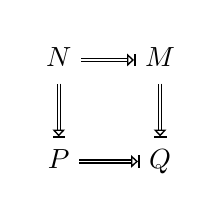
\begin{tikzpicture}
	\matrix (m) [matrix of math nodes] {
	  \trm{N} &[20pt] & \trm{M} \\[20pt] \\ \trm{P} && \trm{Q} \\
	};
	\draw[rwc] (m-1-1) -- (m-1-3);
	\draw[rwc] (m-1-1) -- (m-3-1);
	\draw[rwc] (m-1-3) -- (m-3-3);
	\draw[rwc] (m-3-1) -- (m-3-3);
\end{tikzpicture}}}
&
\vcenter{\hbox{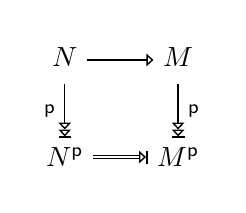
\begin{tikzpicture}
	\matrix (m) [matrix of math nodes] {
	  \trm{N} &[20pt] & \trm{M} \\[20pt] \\ N^\prob && M^\prob \\
	};
	\draw[rw]  (m-1-1) -- (m-1-3);
	\draw[rwn] (m-1-1) --node[left] {$\scriptstyle\prob$} (m-3-1);
	\draw[rwn] (m-1-3) --node[right]{$\scriptstyle\prob$} (m-3-3);
	\draw[rwc] (m-3-1) -- (m-3-3);
\end{tikzpicture}}}
\\ \\
  \text{Lemma~\ref{lem:parallel p - parallel beta}}
& \text{Lemma~\ref{lem:exhaustive p - parallel beta}}
& \text{Lemma~\ref{lem:complete diamond}}
& \text{Lemma~\ref{lem:p to complete reduction}}
\end{array}
\]



\[
\begin{array}{l}
	N\rw M
\\
	N\rws M
\\
	N\rwn M
\\
	N\rwp M
\end{array}
\]

\bibliographystyle{plain}
\bibliography{biblio}
\addcontentsline{toc}{section}{References}

\end{document}

%============================================================
